La libreria \jointjs{} è una libreria per diagrammi scritta in JavaScript e sviluppata da clientIO (\url{client.io}). Essa è open-source, licenziata sotto Mozilla Public License.

Tra alcune funzionalità più di nota si trovano:
\begin{itemize}
	\item elementi per diagrammi base (e.g. rettangoli, cerchi, testo, immagini);
	\item diagrammi già pronti all'uso;
	\item elementi custom basati su SVG;
	\item elementi (\texttt{Elements}) e collegamenti (\texttt{Link}) interattivi;
	\item collegamenti personalizzabili (punta, etichette);
	\item arrotondamento dei collegamenti (con interpolazioni di bezier);
	\item elementi magnetici;
	\item diagrammi gerarchici;
	\item serializzazione/deserializzazione con JSON;
	\item altamente event-driven;
	\item zoom in/out;
	\item supporto a dispositivi touch;
	\item architettura MVC (da \backbonejs).
\end{itemize}

\begin{figure}[H]
	\makebox[\textwidth][c]{
	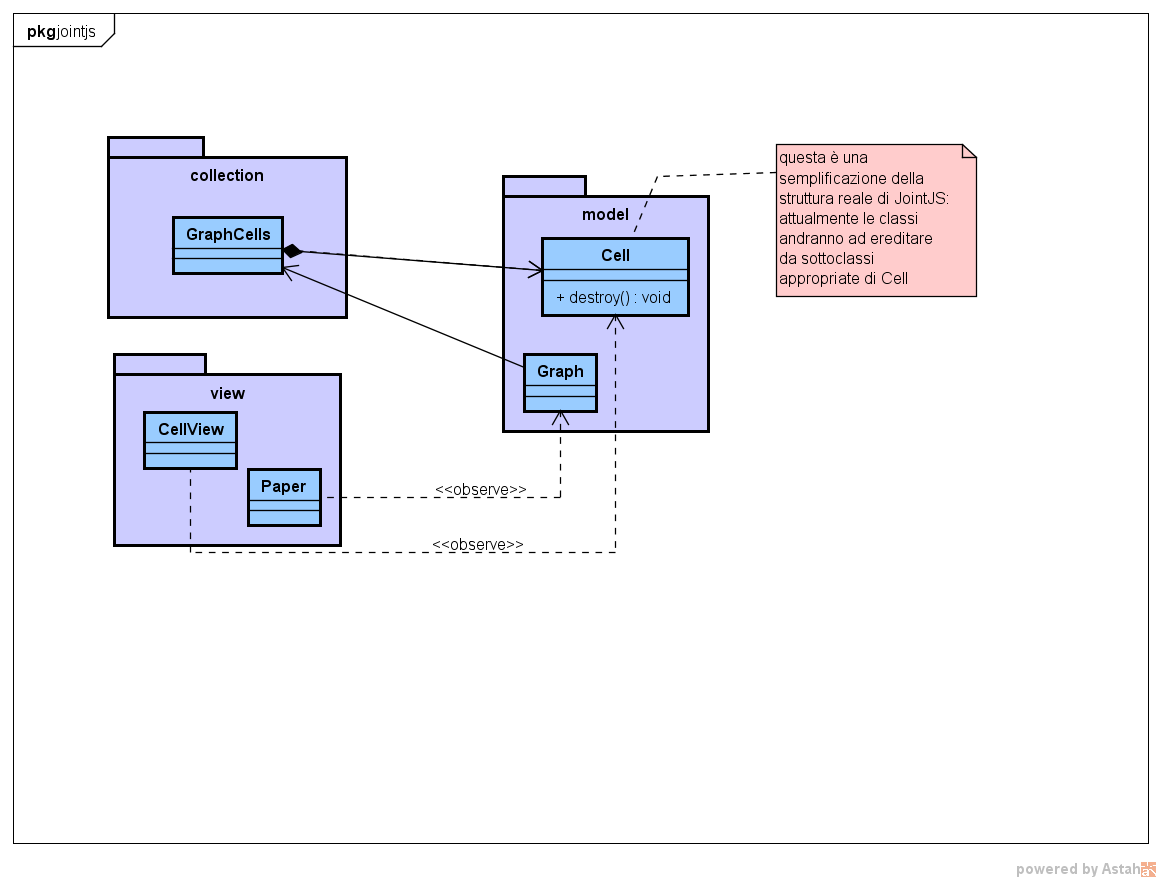
\includegraphics[width=1\textwidth]{img/jointjs}}
	\caption{Esemplificazione delle classi di \jointjs.}
\end{figure}

La figura precedente mostra una esemplificazione della gerarchia di classi usata da \proj. Essa mostra tre package distinti, model, view e collection, per indicare che essi derivano da \texttt{Backbone.Model}, \texttt{Backbone.View} e \texttt{Backbone.Collection} rispettivamente.

La creazione di un nuovo diagramma è piuttosto semplice: è sufficiente specificare un \texttt{Graph} sul quale un \texttt{Paper} deve rimanere in ascolto (\emph{observe}). È possibile catturare eventi all'interno del \texttt{Paper} e gestirli di conseguenza.

Il \texttt{Graph} possiede al suo interno una \texttt{GraphCells}. Questa rappresenta il raccoglitore di celle (\texttt{Cell}, che costituiscono gli elementi da cui è composto un \texttt{Graph}. 

Una \texttt{Cell} è osservata da una \texttt{CellView} del tutto simile in funzionamento a quanto descritto in precedenza tra un model ed una view. 

Ereditando da \texttt{Cell} (o meglio, dalle appropriate sottoclassi) possiamo disporre già di svariati metodi già implementati e testati da \jointjs{}.
